\begin{figure}[t]
  \centering
  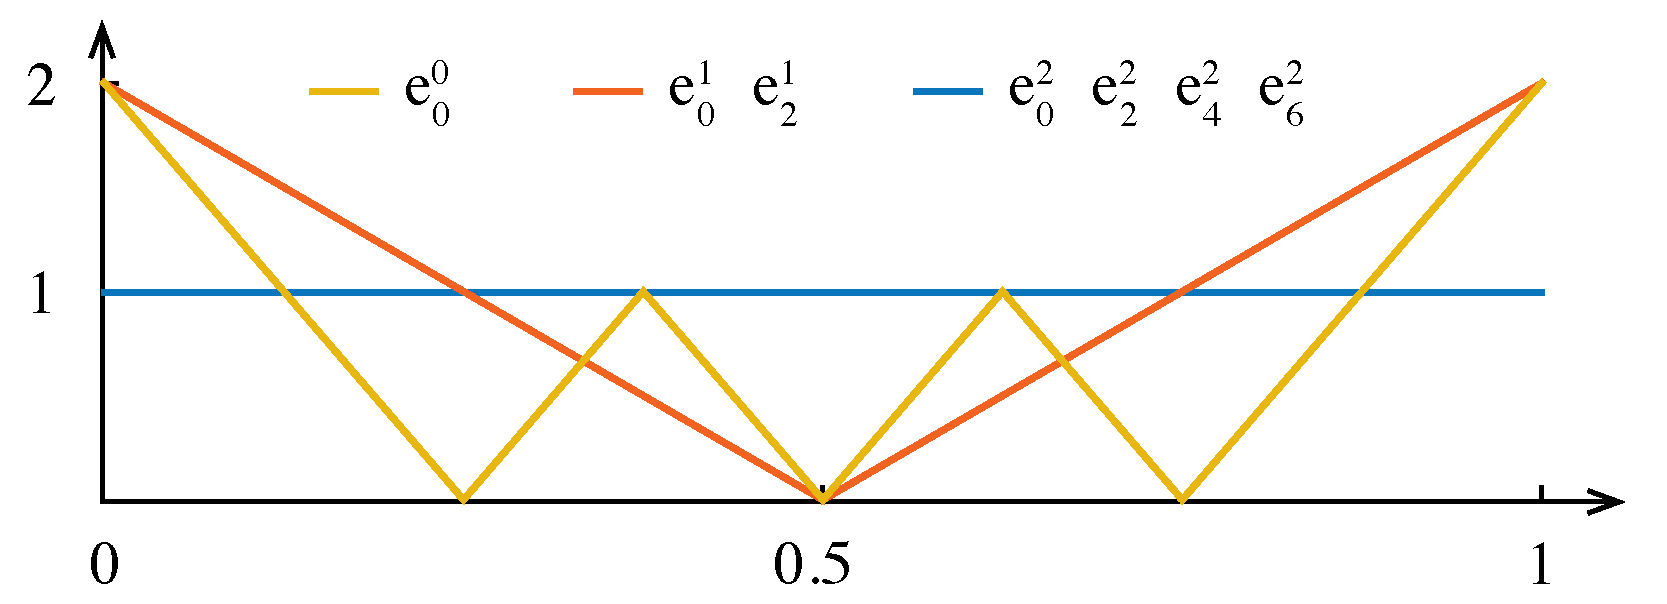
\includegraphics[width=1.0\columnwidth]{include/assets/figures/basis.pdf}
  \vspace{-1.5em}
  \caption{
    The first three levels of the basis described in \sref{basis}.
  }
  \flab{basis}
\end{figure}

The basis functions that go hand in hand with the open Netwon--Cotes rule are
formed by the linear hat function and are as follows \cite{klimke2006}. For $i =
0$ and $j = 0$,
\[
  \e_{00}(\x) = 1.
\]
For $i > 0$ and $j = 0$ (close to the left endpoint),
\[
  \e_{i0}(\x) = \begin{cases}
    2 - \left( \n_i + 1 \right) \x, & \text{if } \x < \frac{2}{\n_i + 1}, \\
    0, & \text{otherwise}.
  \end{cases}
\]
For $i > 0$ and $j = \n_i - 1$ (close to the right endpoint),
\[
  \e_{i(\n_i - 1)}(\x) = \begin{cases}
    \left( \n_i + 1 \right) \x - \n_i + 1, & \text{if } \x > \frac{\n_i - 1}{\n_i + 1}, \\
    0, & \text{otherwise}.
  \end{cases}
\]
In other cases,
\[
  \e_{ij}(\x) = \begin{cases}
    1 - \left( \n_i + 1 \right)|\x - \x^i_j|, & \text{if } |\x - \x^i_j| < \frac{1}{\n_i + 1}, \\
    0, & \text{otherwise}.
  \end{cases}
\]
The basis functions corresponding to the first three levels of one-dimensional
interpolation are depicted in \fref{basis}. Note that $\e_{11}$, $\e_{21}$,
$\e_{23}$, and $\e_{25}$ are not depicted as they are not involved in the
hierarchical construction. In multiple dimensions, the basis functions are
formed as shown in \eref{basis-functions}.

To conclude, all the pieces of the interpolation technique that our framework
makes use of have been introduced. In the next subsection, we would like to give
an algorithmic structure of the technique in order to streamline its
implementation.
